\section{Lessons from Applying the Selected Practice}
\label{sec:Lessons from Applying the Selected Practice}

\subsection{What I Did}
\label{sub:What I Did}


Despite my initial plan being to set up and host most of my Continuous
Integration infrastructure myself, it became clear after an initial trial
that it would be far easier for me to ensure build repeatability/speed if I used
a cloud-based CI service (some of the reasons for which are detailed below).
With this in mind, I elected to use the popular and
excellent \href{https://travis-ci.org/}{Travis CI} - which provides a free tier
for open-source projects such as mine. Setup was as simple as adding a
`.travis.yml` file to my project, and enabling my GitHub repo for builds on
the Travis CI admin panel. My initial .travis.yml file can be seen in
Listing~\ref{lst:initialTravis}, and the latest version is available
\href{https://github.com/FireEater64/gamq/blob/master/.travis.yml}{on GitHub}.
There are a multitude of configurable options available, but
my initial configuration in Listing~\ref{lst:initialTravis} consisted of
only three:

\begin{description}
  \item[Language] Defines the language of the project being built - in this case
  \href{https://golang.org/}{GoLang}. TravisCI builds (usually) take place
  inside \href{https://www.docker.com/what-docker}{Docker containers}, with the
  'language' section of configuration dictating which pre-built container is used for
  this particular build. In this case, a language value of 'go' will ensure that the
  build container contains all of the binaries and environment variables required
  for building and running GoLang projects.
  \item[Go] This section defines different versions of the go compiler you wish
  to build your product on. When code is checked in - Travis will spin up a
  separate container for each version specified, and run your complete test suite
  inside each container in parallel. This feature is known as the
  '\href{https://docs.travis-ci.com/user/customizing-the-build/#Build-Matrix}{build matrix}',
  and is both \emph{incredibly} useful for ensuring software consistency on multiple
  different compilers/runtimes (especially useful for interpreted languages such
  as Java), and something which would be hard to replicate outside of a
  containerised build environment (i.e. if I'd chosen to self-host my CI).
  \item[Script] Any custom commands you wish to be run as part of the build.
  Travis contains (pun intended) a standard build script for most languages (which
  are selected via the 'language' configuration detailed above), however builds
  invariably require additional scripts/commands to be run as well - some example
  use cases could be to run additional tests, or deploy build binaries to an
  artefact repository. In this case, the commands I specified execute both my
  unit/integration test suite, and my benchmark suite (more details below).
\end{description}

More information on the contents of .travis.yml files can be found in their
\href{https://docs.travis-ci.com/}{excellent documentation}.

\begin{listing}
  \centering
  \begin{minted}[frame=single,framesep=10pt]{YAML}
language: go

go:
  - 1.3
  - 1.4
  - tip

script: go test -v ./... -bench=.
  \end{minted}
  \caption{Initial .travis.yml}
  \label{lst:initialTravis}
\end{listing}

Of course, this is only half the story. Using Continuous Integration to ensure
that software builds successfully, whilst useful, does not ensure the correctness
of the software being built. That requires a battery of tests, which can be run
on each successful build, to help ensure the correctness of my project - as well
as help guard against possible regression. The unit/integration/benchmark tests
for my project can be viewed in
\href{https://github.com/FireEater64/gamq}{my projects Git repository}, and uses
the GoLang convention of treating all source files of pattern '*\_test.go' as test
files. The specifics of my test harness are outside the scope of my report, which
deals with my use of Continuous Integration - as a result, only a brief summery of
tests is given.

My tests fall into two main categories, and use the standard, built in testing
features of Go:

\subsubsection{Unit/Integration Tests}
\label{subs:Unit/Integration Tests}

Unit/integration tests in go are written in much the same as any other language
(see Listing~\ref{lst:goUnitTest}) - and afford me protection against code that
fails to meet specification, as well as regressions in functionality resulting
from code changes/re-factoring. One important (though not definitive) metric
associated with unit/integration tests is \emph{code coverage}, which is the
total percentage of the code-base that is executed when running unit tests. This
is a useful metric to keep an eye on, as it helps\footnote{Though doesn't always}
indicate which sections of code are susceptible to bugs as a result of not being
tested. Go's built in test runner is capable of producing code coverage reports
during test runs, however I chose to use an open source tool called '\href{}{gocov}',
as it allowed me to send the code quality metrics produced my build to another
online service, \href{https://coveralls.io/}{coveralls}. The reasons behind doing
this, rather than relying on the build-in HTML report were:

\begin{description}
  \item[Visibility] Publishing my code quality metrics in an easily accessibly,
  publicly visible website (as well as the front page of my GitHub project),
  rather than hiding them away in build logs helps to
  'keep me honest', as well as 'gamify' the process of driving up coverage.
  \item[Monitoring] Coveralls allows me to set 'thresholds' for coverage metrics,
  and will fail the build if these are not adhered to. For example, my build will
  fail if the coverage of the checked in code is even 0.1\% less than that of the
  previous successful build.
\end{description}

The code quality metrics for my project are available
\href{https://coveralls.io/github/FireEater64/gamq?branch=master}{on Coveralls},
as well as being summarised in the
\href{https://github.com/FireEater64/gamq/blob/master/README.md}{README for my
project on GitHub}\(Figure~\ref{fig:readmeStatus} \).

\begin{listing}
\centering
  \begin{minted}[frame=single,framesep=10pt]{Go}
func Test(t *testing.T) {
	underTest := MyClass{}
	result := underTest.SomeFunction()

	if result != expected {
		t.Fail()
	}
}
  \end{minted}
  \caption{An example of a unit test in Go}
  \label{lst:goUnitTest}
\end{listing}

\begin{figure}
  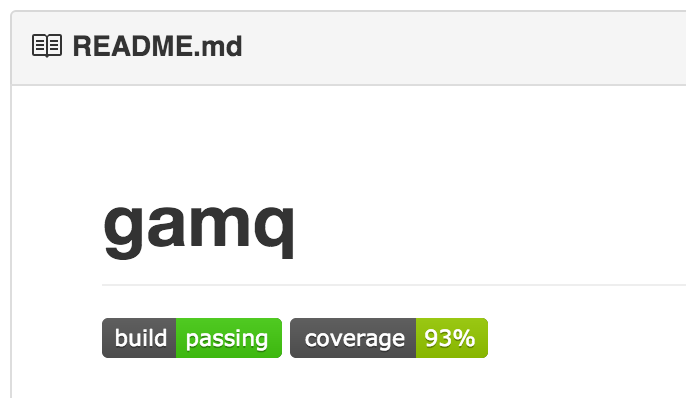
\includegraphics{README}
  \centering
  \caption{Code status badges in README.md}
  \label{fig:readmeStatus}
\end{figure}

\subsubsection{Benchmarks}
\label{subs:Benchmarks}

As well as ensuring the correctness of the code I check in, monitoring changes in
performance for certain critical sections of code is also a concern, when building
a system where speed is required. In order to do this, I used the built-in GoLang
test framework's benchmark support\footnote{Details about which can be found in
the \href{https://golang.org/pkg/testing/}{testing package documentation}} to produce
stable execution times for critical functions.

\begin{listing}
  \centering
  \begin{minted}[frame=single,framesep=10pt]{Go}
func BenchmarkMessageQueue_Push(t *testing.B) {
	underTest := NewMessageQueue()
	testString := "test"

	for i := 0; i < t.N; i++ {
		underTest.Push(&testString)
	}
}
  \end{minted}
  \caption{An example of a benchmark in Go}
  \label{lst:goBenchmark}
\end{listing}

For example,
Listing~\ref{lst:goBenchmark} shows a benchmark function to evaluate the execution time
of the \mintinline{Go}{Push()} function for my MessageQueue implementation. When
run as part of my continuous integration build, the following output
(Listing~\ref{lst:goBenchmarkOutput}) is given for each benchmark. These results
can then be compared across run, with the (still to be implemented) option of
failing the build in the event that a major increase in average execution time
for certain methods is detected, when compared to the previous build (in a similar)
manner to my code coverage metrics. Furthermore, metrics such are this can be
graphed at the end of my project, as one way of (hopefully) illustrating the
fact that my codebase has slowly improved over time.

\begin{listing}
  \centering
  \begin{minted}[frame=single, framesep=10pt]{Bash}
BenchmarkMessageQueue_Push-2 # Benchmark Name
5000000 # Number of times loop executed to get a stable average
239 ns/op # Average execution time across all runs
  \end{minted}
  \caption{Example benchmark output}
  \label{lst:goBenchmarkOutput}
\end{listing}

\subsection{What I Learned}
\label{sub:What I Learned}

Despite my having experience using Continuous Integration on large software
projects, I still feel that this exercise has taught me much.

My previous experiences with Continuous Integration were largely based around
enterprise-scale, in house \href{https://www.jetbrains.com/teamcity/}{TeamCity}
deployments. There are several pros and cons to this approach:

\begin{itemize}
  \item[\textcolor{green}{$\bullet$}] Complete control over the build flow/build agent configuration
  \item[\textcolor{green}{$\bullet$}] Hosted internally, so builds can contain
  sensitive information (API Keys/propriatry code etc.)
  \item[\textcolor{red}{$\bullet$}] Difficult to scale dynamically
  (have to configure additional build agents)
  \item[\textcolor{red}{$\bullet$}] Slow to get started with - very little
  configuration out of the box
  \item[\textcolor{red}{$\bullet$}] Limited integration with other (non-JetBrains)
  services
\end{itemize}

My initial attempts at continuous integration followed this pattern, using
a self-hosted instance of \href{http://jenkins-ci.org/}{Jenkins CI}
(Figure~\ref{fig:jenkinsDashboard} ) to build early versions of my project,
final report and seminar presentation\footnote{Both of which were written in
\LaTeX. My CI builds for these projects builds and spell checks the latest
versions of the code, and send the completed report to my
supervisor}.

\begin{figure}
  \noindent\makebox[\textwidth]{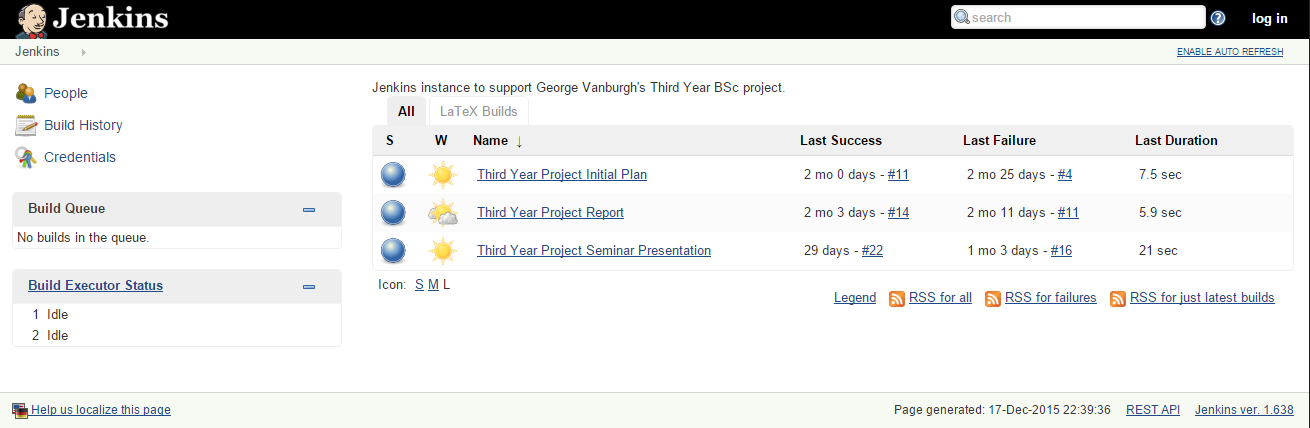
\includegraphics[width=\textwidth]{Jenkins}}
  \centering
  \caption{Jenkins build dashboard}
  \label{fig:jenkinsDashboard}
\end{figure}

Shortly after setting up my intiial project build, however, I began to run into
issues with managing my own build infrastructure (some of which are outlined
above) which lead me to look into using a hosted solution like TravisCI as an
alternative. In contrast to the above points:

\begin{itemize}
  \item[\textcolor{green}{$\bullet$}] Very little configuration required to get
  set up (as shown in Section~\ref{sub:What I Did})
  \item[\textcolor{green}{$\bullet$}] Powerful, easily configurable integration
  with other web services, such as Coveralls
  (discussed in Section~\ref{sub:What I Did}) and \href{https://pushover.net/}{Pushover}
  (which I used for build success/failure notifications)
  \item[\textcolor{green}{$\bullet$}] Easy to scale, as a result in running (most)
  builds inside Docker containers - which are spun up on demand - Travis allows
  for several builds to be executed at the same time, which shortens the feedback
  loop after checking in code.
  \item[\textcolor{green}{$\bullet$}] Very little to self-manage. By removing the
  need to maintain/manage build servers - a (surprisingly large) chunk of time is
  saved, allowing me to focus more on my code/tests, rather than my build infrastructure.
  \item[\textcolor{green}{$\bullet$}] Tight integration with GitHub, which allows
  me to
  \href{https://github.com/FireEater64/gamq/releases}{publish build artifacts as part of a Travis build},
  and automatically build/test any pull requests I receive in the future (none yet sadly).
  \item[\textcolor{red}{$\bullet$}] Public infrastructure, so uploading sensitive
  data/code, private keys, passwords etc. is not a good idea. Fortunately, what little
  information I do need to upload (such as my \href{https://github.com/FireEater64/gamq/blob/aabc34061b46f5b743d62681e8d19a74c907ec83/.travis.yml#L27}{GitHub API key for pushing build artifacts}
  can be \href{https://docs.travis-ci.com/user/encryption-keys/}{encrypted}.)
  \item[\textcolor{red}{$\bullet$}] Limited control over build agent configuration. Currently,
  users have no control over the base TravisCI container/VM image. It is, however
  completely possible to install/configure additional software at build time
  (although this can inrease the build time significantly/lead to bloated build scripts).
  Refer to the \href{https://docs.travis-ci.com/user/ci-environment/#Virtualization-environments}{Travis documentation}
  for more information.
\end{itemize}

One other frequently cited concern with using a cloud-based CI provider, is that
these services can be unreliable/are outside of your control. Whilst it's true
that online services have suffered several (high-profile) outages in the past,
my personal view (and one which is backed by several months of flawless service)
is that the engineering expertise of companies like Travis are capable of producing
a service reliable enough for the majority of open source projects/myself
(and that is certainly more reliable than any service I could roll myself - as per
my server uptime in Figure~\ref{georgeServeUptime}).

\begin{figure}
  \noindent\makebox[\textwidth]{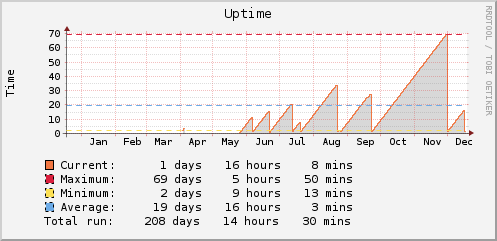
\includegraphics[width=\textwidth]{GeorgeServeUptime}}
  \centering
  \caption{My attempts at keeping a server online}
  \label{fig:georgeServeUptime}
\end{figure}

I ended up switching my build to TravisCI for the above reasons\footnote{For my
main project build - my \LaTeX builds are staying on Jenkins
(at least in the short term), due to limited *Tex support from TravisCI}, and
couldn't be happier with how it's worked for me.
